\documentclass[11pt,a4paper]{article}

\usepackage[a4paper,left=1.35in,right=1.35in,top=1.25in,bottom=1.05in]{geometry}
\usepackage{times}
\usepackage{setspace}
\usepackage{graphicx}
\usepackage{array}
\usepackage{booktabs}
\usepackage{longtable}
\usepackage{tabularx}
\usepackage{enumitem}
\usepackage{float}
\usepackage{caption}
\usepackage{hyperref}
\usepackage{xcolor}
\usepackage{tikz}
\usepackage{titlesec}
\usetikzlibrary{arrows.meta,positioning,shapes.geometric}

\hypersetup{
    colorlinks=true,
    linkcolor=black,
    citecolor=black,
    urlcolor=black,
    pdftitle={Site Meeting Copilot v2 Research Paper},
    pdfauthor={Kalla Lokaditya}
}

\setstretch{1.08}
\setlength{\parindent}{17pt}
\setlength{\parskip}{4pt}
\sloppy

\titleformat{\section}
  {\normalfont\Large\bfseries}{\thesection}{1em}{}
\titleformat{\subsection}
  {\normalfont\large\bfseries}{\thesubsection}{1em}{}
\titleformat{\subsubsection}
  {\normalfont\normalsize\bfseries}{\thesubsubsection}{1em}{}
\captionsetup{font=small,labelfont=bf}

\newcolumntype{Y}{>{\raggedright\arraybackslash}X}

\begin{document}

\begin{center}
    \vspace*{1.1cm}
    {\LARGE\bfseries A Local AI Framework for Construction Site Meeting Minutes Generation Using Whisper Transcription and Structured LLM Analysis\par}
    \vspace{1.0cm}
    {\large Kalla Lokaditya$^{1*}$\par}
    \vspace{0.55cm}
    {$^{1}$Department of Computer Science and Engineering, Dayananda Sagar University, Bengaluru, Karnataka, India.\par}
    \vspace{0.25cm}
    {*Corresponding author. USN: ENG23CS0570. E-mail: ENG23CS0570@dsu.edu.in\par}
\end{center}

\vspace{1.1cm}

\begin{center}
    \textbf{Abstract}
\end{center}

\noindent Construction site meetings produce important decisions, blockers, responsibilities, due dates, safety observations and schedule changes. In many small and medium construction projects, this evidence is captured as unstructured audio, handwritten notes, messaging app updates or spreadsheet revisions. Manual preparation of meeting minutes and action trackers is time consuming, and missing a single dependency can delay procurement, site execution or client communication. This paper presents Site Meeting Copilot v2, a local AI-based framework that converts construction site meeting evidence into structured and reviewable project governance outputs. The system accepts meeting audio or pasted transcript text, agenda text and a project schedule CSV. A local Flask Whisper server transcribes supported audio files, while Ollama with the phi3:mini language model analyses the transcript with agenda and schedule context. The framework extracts summaries, decisions, blockers, risks, action items, owners, due dates, agenda coverage and schedule impact flags. Outputs are displayed in a browser dashboard and can be exported as meeting minutes, an action tracker and a schedule impact report. The Version 1 implementation was evaluated using functional tests for audio upload, transcription server health, malformed schedule input, agenda matching, JSON extraction and report generation. The results show that a local AI pipeline can support site engineers by transforming unstructured meeting discussions into actionable project records while keeping the human user in control of review and approval.

\newpage

\noindent\textbf{Keywords:} Construction Site Meetings, Meeting Minutes, Automatic Speech Recognition, Whisper, Local Large Language Models, Ollama, Action Tracker, Schedule Impact Analysis, Project Governance, Construction AI.

\section{Introduction}

Construction projects depend on repeated coordination among owners, project managers, site engineers, consultants, contractors, suppliers and safety teams. Site meetings are used to review progress, identify blockers, approve decisions, assign responsibilities and resolve dependencies between work packages. Although these meetings are operationally important, the records generated during them are often incomplete or scattered across multiple informal sources. A single project decision may appear in a meeting recording, a WhatsApp message, an Excel schedule, a site diary and a later follow-up call. This fragmentation makes it difficult for teams to maintain a reliable project memory.

The preparation of meeting minutes is therefore an important but time-consuming activity. A site engineer may attend the meeting, make notes, inspect drawings, verify the schedule and later prepare a minutes of meeting document. If the meeting is long or contains many stakeholders, action items can be missed. If the schedule impact is not identified early, the project team may discover delays only after downstream work has already been affected. This problem is especially relevant in construction, where delayed materials, safety observations, access constraints, manpower shortages and blocked work fronts can quickly affect linked activities.

Recent progress in automatic speech recognition and local language models makes it possible to support this workflow using AI. Whisper-style transcription can convert audio into text, while compact language models can extract structured fields from the transcript. However, a normal meeting summarizer is not sufficient for a construction site workflow. A site meeting system should not simply produce a paragraph summary. It should identify decisions, blockers, owners, deadlines, agenda coverage and potential schedule impact. It should also allow the user to review the transcript and generated outputs because construction decisions require accountability.

Site Meeting Copilot v2 applies these capabilities to the construction meeting domain. The system works as a local prototype that accepts meeting audio or transcript text, agenda text and a project schedule CSV. It performs transcription using a local Whisper server, analyses the meeting using a local language model through Ollama, and renders structured outputs in a browser dashboard. The project is intended as a Version 1 release of a construction meeting intelligence assistant. It focuses on converting a meeting into reliable records: meeting minutes, action tracker entries and schedule impact indicators.

The contribution of this paper is an integrated framework for local construction meeting intelligence. The framework links local transcription, structured LLM extraction, agenda cross-reference checking and schedule impact analysis in a single workflow. The design keeps the transcript editable and the outputs reviewable because AI-generated meeting records should support a site engineer rather than replace professional judgement. The paper also maps the implemented features to Version 1 requirements and discusses how the same project can evolve into a larger construction AI operating system.

\section{Literature Survey}

The literature survey is presented in the same table-based format used in the sample research paper. The selected works are existing reference papers and studies related to construction meeting documentation, artificial intelligence in construction, speech recognition, meeting summarization, large language models and compact local models.

\begingroup
\small
\renewcommand{\arraystretch}{1.16}
\setlength{\tabcolsep}{5pt}
\begin{longtable}{p{0.9cm}p{5.0cm}p{1.1cm}p{5.4cm}}
\toprule
\textbf{Ref.} & \textbf{Paper} & \textbf{Year} & \textbf{Relevance to Your Work} \\
\midrule
\endfirsthead

\toprule
\textbf{Ref.} & \textbf{Paper} & \textbf{Year} & \textbf{Relevance to Your Work} \\
\midrule
\endhead

\cite{constructionmeetings} & Meetings Critical to Construction Project Success and Best Practices: A Case Study -- Ludwig & 2018 & Directly relevant to the construction domain because it explains the importance of site meetings, clear documentation and follow-up in construction project success. It supports the need for a system that converts meeting discussion into reliable project records. \\

\cite{abioye} & Artificial Intelligence in the Construction Industry: A Review of Present Status, Opportunities and Future Challenges -- Abioye et al. & 2021 & Relevant to the broader Construction AI direction of the project. The paper shows that AI can support planning, risk management, safety and project control, which are all connected to the meeting intelligence workflow of Site Meeting Copilot v2. \\

\cite{pan2021} & Roles of Artificial Intelligence in Construction Engineering and Management: A Critical Review and Future Trends -- Pan and Zhang & 2021 & Supports the construction engineering and management scope of the project. It shows how AI can assist decision-making, planning and management tasks in construction projects. \\

\cite{baduge2022} & Artificial Intelligence and Smart Vision for Building and Construction 4.0: Machine and Deep Learning Methods and Applications -- Baduge et al. & 2022 & Relevant because it reviews AI, ML and deep learning applications across the building and construction lifecycle, including construction management, progress monitoring and safety. \\

\cite{ghimire2023} & Generative AI in the Construction Industry: Opportunities and Challenges -- Ghimire, Kim and Acharya & 2023 & Closely related to the future scope of the project because it discusses how generative AI can be introduced into construction workflows and what challenges must be addressed. \\

\cite{whisper} & Robust Speech Recognition via Large-Scale Weak Supervision -- Radford et al. & 2023 & Highly relevant to the audio processing layer of the project. It supports the use of Whisper-style automatic speech recognition for converting construction meeting recordings into editable transcript text. \\

\cite{icsi} & The ICSI Meeting Corpus -- Janin et al. & 2003 & Relevant to meeting transcription research because it provides a natural meeting corpus for studying multiparty speech, meeting audio and spoken interaction. \\

\cite{ami} & The AMI Meeting Corpus -- Carletta et al. & 2005 & Relevant because it provides a multimodal meeting corpus and supports research on meeting capture, meeting transcription and meeting understanding. \\

\cite{qmsum} & QMSum: A New Benchmark for Query-Based Multi-Domain Meeting Summarization -- Zhong et al. & 2021 & Relevant to the meeting analysis component. The paper shows that meeting users often need different outputs from the same meeting, supporting this project's separation of summary, decisions, blockers, action items and schedule impact. \\

\cite{nallapati2016} & Abstractive Text Summarization Using Sequence-to-Sequence RNNs and Beyond -- Nallapati et al. & 2016 & Supports the summarization layer of the project by showing how neural models can generate concise summaries from longer text inputs. \\

\cite{bart2020} & BART: Denoising Sequence-to-Sequence Pre-training for Natural Language Generation, Translation, and Comprehension -- Lewis et al. & 2020 & Relevant to modern text generation and summarization. It supports the idea that pretrained sequence-to-sequence models are effective for generating summaries from unstructured text. \\

\cite{llmsurvey} & A Survey of Large Language Models -- Zhao et al. & 2023 & Relevant to the structured LLM analysis part of the system. It supports the use of LLMs for summarization, instruction following and information extraction from unstructured meeting transcripts. \\

\cite{brown2020} & Language Models are Few-Shot Learners -- Brown et al. & 2020 & Supports prompt-based language model usage. It is relevant because Site Meeting Copilot v2 depends on prompt instructions to extract structured fields from meeting transcripts. \\

\cite{sbert} & Sentence-BERT: Sentence Embeddings Using Siamese BERT-Networks -- Reimers and Gurevych & 2019 & Relevant to semantic matching and future agenda-cross-reference improvements, where agenda items and transcript segments can be compared using sentence-level semantic similarity. \\

\cite{phi3} & Phi-3 Technical Report: A Highly Capable Language Model Locally on Your Phone -- Abdin et al. & 2024 & Relevant to the local AI design of the project. It supports the idea that compact language models can run locally, which matches the project's Ollama and phi3:mini based implementation. \\
\bottomrule
\end{longtable}
\endgroup

From the above survey, the research gap is clear: existing works discuss construction meetings, AI in construction, speech recognition, meeting summarization and LLMs separately. Site Meeting Copilot v2 combines these areas into a single construction-focused workflow that accepts meeting audio, generates an editable transcript, extracts structured meeting minutes, identifies action items and flags possible schedule impacts.

\section{Proposed Methodology}

The proposed methodology follows a pipeline approach. The user provides meeting evidence and context. The system transcribes audio if required, builds an analysis prompt, requests structured output from the local language model, validates the response and renders it in the dashboard.

The methodology is designed around a Version 1 release of a construction meeting intelligence system. The purpose of this release is not to replace enterprise construction management software. Instead, it proves the core workflow required for a useful site meeting assistant: accept meeting evidence, convert audio into transcript text, analyse the meeting, detect agenda coverage, identify schedule-related issues and export reviewable project records. This scoped approach makes the system practical for an engineering student project while keeping the design open for later expansion.

The project follows a human-in-the-loop methodology. The system does not directly approve decisions, change the schedule or send messages to contractors. It generates structured outputs and allows the user to review them. This choice is important because construction meeting records may affect responsibility, cost and safety. A human site engineer must remain the final authority before generated minutes or action trackers are shared.

\begin{figure}[H]
\centering
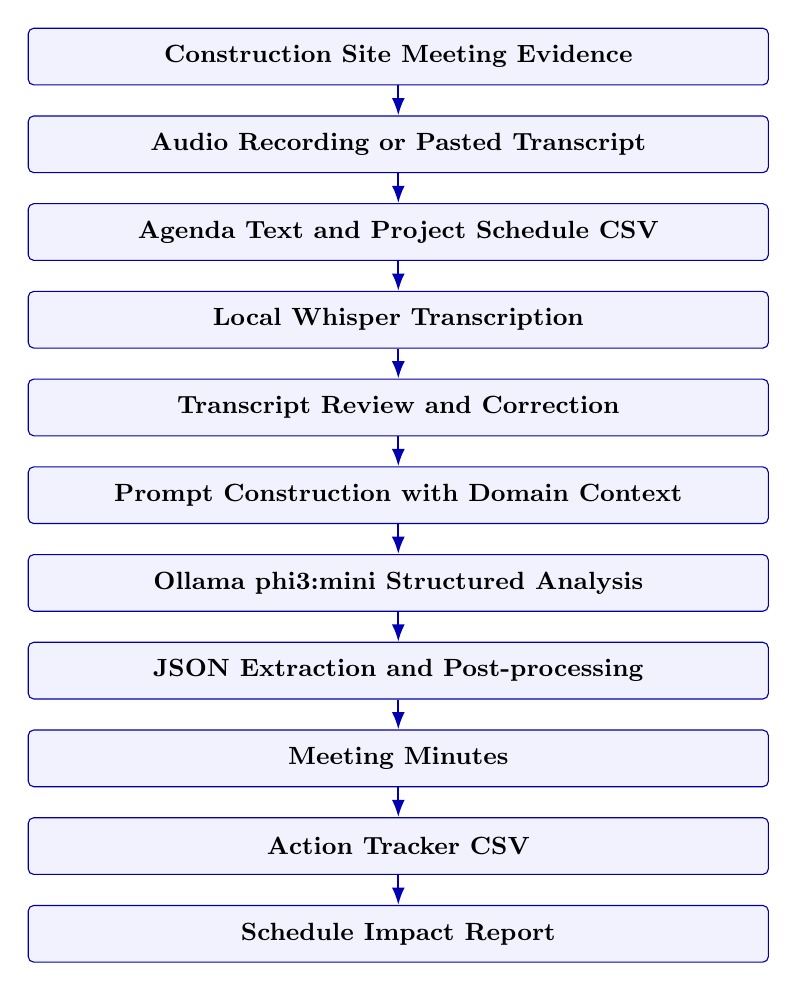
\begin{tikzpicture}[
    node distance=0.38cm,
    process/.style={draw=blue!65!black, rounded corners=2pt, fill=blue!5, align=center, minimum width=9.4cm, minimum height=0.72cm, text width=9.1cm, font=\small\bfseries},
    arrow/.style={-{Latex[length=2.2mm]}, thick, draw=blue!70!black}
]
\node[process] (a) {Construction Site Meeting Evidence};
\node[process, below=of a] (b) {Audio Recording or Pasted Transcript};
\node[process, below=of b] (c) {Agenda Text and Project Schedule CSV};
\node[process, below=of c] (d) {Local Whisper Transcription};
\node[process, below=of d] (e) {Transcript Review and Correction};
\node[process, below=of e] (f) {Prompt Construction with Domain Context};
\node[process, below=of f] (g) {Ollama phi3:mini Structured Analysis};
\node[process, below=of g] (h) {JSON Extraction and Post-processing};
\node[process, below=of h] (i) {Meeting Minutes};
\node[process, below=of i] (j) {Action Tracker CSV};
\node[process, below=of j] (k) {Schedule Impact Report};
\foreach \x/\y in {a/b,b/c,c/d,d/e,e/f,f/g,g/h,h/i,i/j,j/k}
    \draw[arrow] (\x) -- (\y);
\end{tikzpicture}
\caption{Workflow of the proposed local AI-based construction site meeting intelligence system.}
\end{figure}

\subsection{Input Acquisition}

The system accepts four categories of input. The first is an audio recording of the site meeting. The second is transcript text, which may be pasted directly if the meeting has already been transcribed. The third is the meeting agenda, which lists expected discussion points. The fourth is a project schedule CSV containing activities, owners, planned dates or status information.

This input design is important because meeting understanding improves when the model has context. If the agenda states that concrete curing, material delivery and safety inspection must be discussed, the system can identify which agenda points were covered and which were missed. If the schedule contains linked activities, the system can flag possible impacts from blockers or delays mentioned in the meeting.

The audio input is treated as raw meeting evidence, while the transcript is treated as the editable textual record. This separation is useful because some users may already have a transcript from another source, while others may only have a recording. The system therefore supports both workflows. Agenda and schedule inputs are optional in the sense that the system can still summarize a meeting without them, but they improve the quality and usefulness of the output.

\subsection{Whisper Transcription}

When an audio file is uploaded, the frontend sends it to the Flask Whisper server. The server exposes routes for health checking, model warmup and automatic speech recognition. Supported audio formats include common meeting recording formats such as MP3, WAV, M4A and WebM. After transcription, the server returns text to the frontend. The transcript is not hidden from the user; it is placed in an editable field so that errors can be corrected before analysis.

The editable transcript step is a practical safeguard. A construction meeting may contain names of local contractors, site blocks, material brands, tower numbers or abbreviations. If the speech recognizer mishears any of these terms, direct LLM analysis may produce incorrect action items. Human review between transcription and analysis reduces this risk.

In the Version 1 design, the Whisper service is separated from the frontend. This makes the architecture easier to test because the user can check whether the speech server is running before attempting analysis. It also makes the system easier to upgrade. A future version can replace the transcription model, add speaker diarization or move speech processing into a backend service without redesigning the entire user interface.

\subsection{Agenda Cross-reference}

The agenda cross-reference stage compares the meeting content with the expected agenda items. The system asks the model to determine which agenda topics were discussed, which were partially discussed and which were missed. This feature is valuable because a meeting summary alone cannot tell whether the meeting achieved its purpose. For example, a meeting may generate a useful summary but still fail to discuss safety inspection or procurement follow-up.

This stage also gives the user a simple quality check for the meeting itself. If an agenda item is marked as missed, the project team can schedule a follow-up discussion. If an item is marked as partially discussed, the user can inspect the generated notes and decide whether enough information was captured. In this way, the system supports both documentation and meeting improvement.

\subsection{Structured LLM Analysis}

The LLM analysis stage uses a carefully prepared prompt. The prompt instructs the model to behave like a construction meeting assistant and return machine-readable JSON. The required fields include meeting summary, decisions, blockers, action items, risks, agenda coverage and schedule impact. The prompt also asks for owners, due dates and priority where available. If the information is not present, the model should use an empty value rather than inventing details.

The output is parsed by the frontend. If the model produces extra text around the JSON, the application attempts to extract the JSON block. The parsed structure is then rendered into sections of the dashboard. This approach makes the output more useful than free-form text because each field can be displayed, exported and reviewed separately.

Structured output is one of the main design decisions of the project. A normal paragraph summary may be easy to read, but it is difficult to track. A structured action item can be converted into a CSV row. A structured blocker can be linked to a schedule activity. A structured decision can be reviewed as part of meeting minutes. The JSON format therefore acts as a bridge between natural language discussion and project management records.

\subsection{Prompt and Schema Design}

The prompt is designed to reduce ambiguity. It provides the transcript, agenda and schedule context, then asks the model to extract information using predefined fields. The required schema includes a meeting summary, decisions, blockers, action items, risks, agenda coverage and schedule impact. Each action item should include task description, owner, due date and status when this information is present in the meeting. Each schedule impact should include the affected activity, reason and severity.

The schema is intentionally simple because the Version 1 system uses a compact local model. A very complex schema may reduce reliability. The project therefore chooses fields that are immediately useful to a site engineer and can be reviewed easily in the dashboard. This design also supports future database migration because the same fields can later become database tables for meetings, tasks, risks and decisions.

\subsection{Post-processing and Validation}

After the model returns a response, the frontend performs post-processing. The first step is to locate the JSON structure. If the response contains explanatory text before or after the JSON, the application extracts the JSON block. The second step is to parse the data and assign default values if optional fields are missing. The third step is to render each category in the correct dashboard section.

Validation is necessary because local LLMs may not always follow instructions perfectly. The system therefore treats the model output as a draft. The user can inspect the generated text, compare it with the transcript and decide whether the output is acceptable. This approach is safer than assuming that the AI result is automatically correct.

\subsection{Schedule Impact Analysis}

The schedule CSV is used to identify whether meeting statements may affect project activities. If the meeting mentions a delay in cement delivery and the schedule contains concreting tasks, the system can mark a potential schedule impact. The current implementation is a Version 1 rule-supported and LLM-supported analysis, not a full critical path scheduling engine. Its purpose is to flag possible impacts early so that the engineer can review them.

The schedule impact output is therefore advisory. It helps the user notice possible connections between meeting discussion and project timelines. It does not replace Primavera, MS Project or formal critical path analysis. This limitation is acceptable for Version 1 because the objective is early warning and documentation support. Future versions can integrate dependency graphs, baseline schedules and database-backed project history.

\section{System Architecture and Implementation}

The system architecture has four main layers: frontend layer, speech layer, model layer and output layer. The frontend is implemented using HTML, CSS and JavaScript. It manages file upload, transcript editing, agenda entry, schedule upload and result rendering. The speech layer is implemented as a Flask server running on localhost. The model layer uses Ollama on localhost with phi3:mini. The output layer renders meeting minutes, action tracker tables and schedule impact information.

\begin{figure}[H]
\centering
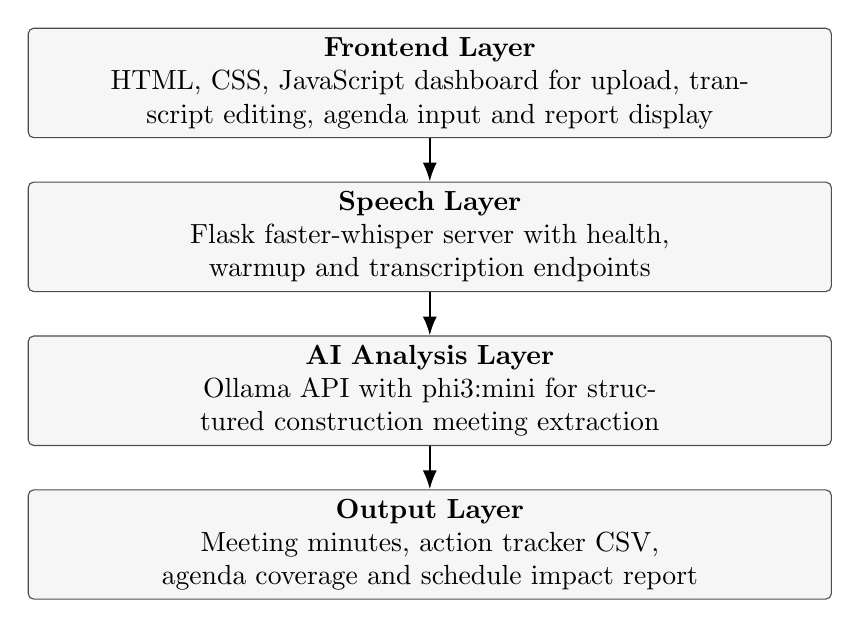
\begin{tikzpicture}[
    layer/.style={draw=black!70, rounded corners=2pt, fill=gray!7, align=center, minimum width=10.2cm, minimum height=1.05cm, text width=9.8cm},
    arrow/.style={-{Latex[length=2.4mm]}, thick}
]
\node[layer] (front) {\textbf{Frontend Layer}\\HTML, CSS, JavaScript dashboard for upload, transcript editing, agenda input and report display};
\node[layer, below=0.55cm of front] (speech) {\textbf{Speech Layer}\\Flask faster-whisper server with health, warmup and transcription endpoints};
\node[layer, below=0.55cm of speech] (model) {\textbf{AI Analysis Layer}\\Ollama API with phi3:mini for structured construction meeting extraction};
\node[layer, below=0.55cm of model] (output) {\textbf{Output Layer}\\Meeting minutes, action tracker CSV, agenda coverage and schedule impact report};
\draw[arrow] (front) -- (speech);
\draw[arrow] (speech) -- (model);
\draw[arrow] (model) -- (output);
\end{tikzpicture}
\caption{Layered architecture of Site Meeting Copilot v2.}
\end{figure}

\subsection{Frontend Dashboard}

The frontend provides the main user interface. It allows the user to upload an audio file, paste transcript text, enter meeting agenda and upload a schedule CSV. After analysis, the dashboard displays the generated output in separate sections. This separation helps the user quickly inspect decisions, blockers, tasks and schedule risks rather than reading a long unstructured paragraph.

The interface also supports export operations. Meeting minutes can be saved as a document-style output, action items can be exported as CSV and schedule impact can be reviewed separately. These exports support practical academic demonstration because the output can be submitted as evidence of system functionality.

The dashboard is organized around the natural workflow of a site engineer. First, the user provides meeting evidence. Next, the user checks or edits the transcript. Then the user runs the AI analysis and reviews the results. This flow reduces confusion because the system does not hide the intermediate transcript. The user can see what information the model is analysing, which improves trust and makes debugging easier during demonstration.

The use of HTML, CSS and JavaScript keeps the Version 1 frontend lightweight. It can be opened and demonstrated without a complex deployment setup. This is suitable for a college project because the main research contribution is the meeting intelligence pipeline, not enterprise frontend infrastructure. At the same time, the frontend is structured in a way that can later be converted into React or Next.js if the project becomes a larger product.

\subsection{Whisper Server}

The Whisper server is implemented in Python using Flask. It provides a health endpoint to confirm whether the server is running, a warmup endpoint to load the model and an ASR endpoint to transcribe uploaded audio. Keeping this server separate from the frontend makes the architecture easier to evolve. A future backend can reuse the same speech service or replace it with a more scalable speech pipeline.

The health endpoint is important for usability. If the Whisper server is not running, the user should know before attempting audio transcription. The warmup endpoint improves the first-run experience because speech models may take time to load. The ASR endpoint performs the actual transcription and returns text to the browser. This service separation makes the project easier to explain during evaluation because each component has a clear responsibility.

\subsection{Ollama Integration}

The frontend communicates with Ollama through the local API. The prompt contains the meeting transcript, agenda and schedule summary. The model is asked to return a JSON object following the expected structure. Since small local models may not always return perfect JSON, the application includes logic to locate and parse the JSON portion of the response. This design is a reasonable Version 1 approach for a student MVP, but production systems should use stricter schema validation and stronger models.

Ollama is used as the local inference layer so that the prototype can run without mandatory cloud API keys. The chosen model, phi3:mini, is small enough to run locally on typical development hardware while still being capable of instruction following. This choice reflects the project requirement of demonstrating a practical local AI system. In future versions, the model layer can be made configurable so that the user can choose between local models and stronger cloud models depending on privacy and performance needs.

\subsection{Output Generation}

The generated outputs are divided into meeting intelligence categories. The summary explains the overall meeting. Decisions record what was approved or agreed. Blockers identify constraints preventing progress. Action items include owner and due date when available. Agenda coverage shows what was discussed and missed. Schedule impact identifies project activities that may be affected. This output design converts meeting evidence into a project control artifact.

Each output category has a practical role. The summary is useful for quick reading. Decisions are useful for accountability. Blockers are useful for escalation. Action items are useful for follow-up. Agenda coverage is useful for checking meeting completeness. Schedule impact is useful for early delay detection. By separating these outputs, the system supports different stakeholders without requiring them to read the full transcript.

\subsection{Export and Review Layer}

The export layer is included because generated information becomes useful only when it can be shared or stored. In the current project, the generated records can be exported as meeting minutes, an action tracker and a schedule impact report. These outputs represent the minimum records expected from a construction meeting intelligence MVP.

The review layer is equally important. The user should not directly circulate AI-generated minutes without checking them. Therefore, the system presents outputs in readable dashboard sections. The user can compare the results with the transcript and identify any mistakes. This design supports responsible AI use in a domain where documentation can affect responsibility and project cost.

\begin{table}[H]
\centering
\caption{Inputs, processing methods and generated outputs in the Version 1 system.}
\begin{tabularx}{\textwidth}{p{3.2cm}Y Y}
\toprule
\textbf{Input Evidence} & \textbf{Processing Method} & \textbf{Generated Output} \\
\midrule
Meeting audio & Local Whisper transcription through Flask server & Editable transcript for user review \\
Transcript text & Prompt construction and LLM analysis & Summary, decisions, blockers and risks \\
Meeting agenda & Agenda cross-reference with transcript & Discussed, partially discussed and missed agenda items \\
Schedule CSV & Schedule parsing and impact detection & Possible schedule impact report \\
LLM JSON response & JSON extraction and dashboard rendering & Minutes, action tracker and exportable records \\
\bottomrule
\end{tabularx}
\end{table}

\section{Version 1 Release Requirement Mapping}

The Version 1 release is defined as a construction meeting intelligence MVP. It must prove that the system can accept meeting evidence, convert audio to transcript, analyse the content and generate structured outputs. Table \ref{tab:reqmap} maps the implemented functions to the release requirements.

\begin{table}[H]
\centering
\caption{Version 1 requirement mapping for Site Meeting Copilot v2.}
\label{tab:reqmap}
\begin{tabularx}{\textwidth}{p{3.4cm}Y p{2.2cm}}
\toprule
\textbf{Requirement} & \textbf{Implementation in Project} & \textbf{Status} \\
\midrule
Audio upload support & Frontend accepts supported audio files and sends them to the Whisper server & Implemented \\
Speech transcription & Flask server uses faster-whisper to transcribe uploaded audio & Implemented \\
Transcript editing & User can review and modify transcript before analysis & Implemented \\
Agenda support & User can enter agenda text for cross-reference & Implemented \\
Schedule CSV support & User can upload project schedule CSV for impact context & Implemented \\
Meeting summary & LLM extracts concise meeting summary & Implemented \\
Decision extraction & LLM identifies decisions from transcript & Implemented \\
Blocker extraction & LLM identifies blockers and risks & Implemented \\
Action tracker & LLM extracts tasks, owners and deadlines where available & Implemented \\
Schedule impact report & System flags possible schedule-related impacts & Implemented \\
Export support & Dashboard supports output export for minutes and trackers & Implemented \\
Local operation & Uses local Whisper server and local Ollama model & Implemented \\
\bottomrule
\end{tabularx}
\end{table}

The mapping shows that the current project satisfies the core Version 1 requirements. The release is not a full enterprise system because it does not yet include authentication, persistent database storage, project-level memory or multi-user roles. However, those features belong to future versions. The Version 1 goal is to convert site meeting evidence into structured and reviewable records, and that goal is achieved.

\section{Algorithmic Workflow}

The algorithmic workflow begins with input collection and ends with report generation. The simplified workflow is shown below.

\begin{verbatim}
Input:
    audio_file OR transcript_text
    agenda_text
    schedule_csv

Process:
    if audio_file is provided:
        transcript = whisper_server.transcribe(audio_file)
    else:
        transcript = transcript_text

    user reviews transcript
    schedule_context = parse_schedule(schedule_csv)
    prompt = build_prompt(transcript, agenda_text, schedule_context)
    raw_response = ollama.generate(model="phi3:mini", prompt=prompt)
    json_result = extract_json(raw_response)
    dashboard.render(json_result)

Output:
    meeting_minutes
    decision_log
    blocker_list
    action_tracker
    agenda_coverage
    schedule_impact_report
\end{verbatim}

The most important part of the workflow is the structured analysis stage. The prompt is designed to reduce hallucination by asking the model to use only the meeting evidence and context. If information is missing, the model should leave the field empty or mark it as not specified. This is important in construction because assigning an incorrect owner or due date may create confusion in the project team.

\section{Demonstration Scenario and Data Flow}

The project was designed around a realistic site meeting scenario. In such a scenario, the site engineer records a coordination meeting involving the project manager, contractors and suppliers. The discussion includes progress review, material delivery, blocked work, pending inspections and responsibilities for the next day. The meeting may not be perfectly structured, and some information may be repeated or discussed informally. This makes it suitable for testing whether the system can convert unstructured discussion into structured records.

\subsection{Meeting Evidence}

The first form of evidence is the meeting recording. This may be recorded using a phone or laptop microphone. The system does not assume studio-quality audio. However, the quality of transcription depends on the clarity of speech and the amount of background noise. The second form of evidence is the transcript. If audio transcription is successful, the transcript is generated automatically. If a transcript already exists, it can be pasted directly into the text area.

The third form of evidence is the agenda. The agenda may contain items such as concrete work status, reinforcement material delivery, electrical conduit work, safety inspection and contractor follow-up. The fourth form of evidence is the schedule CSV. The schedule may contain activity names, planned dates, owners and status. These inputs allow the system to connect discussion points with expected project activities.

\subsection{Expected Outputs}

For the demonstration scenario, the expected output is not only a summary. The system should identify the key meeting outcomes. If the meeting includes a decision to shift plastering work to the next week, the decision should appear in the decision log. If cement delivery is delayed, it should appear as a blocker. If a person is asked to follow up with a vendor, it should appear as an action item with an owner. If an agenda item is not discussed, it should appear in the missed agenda list. If a delay affects a scheduled activity, it should appear in the schedule impact report.

This output structure makes the system suitable for project reviews. A teacher, evaluator or project guide can check whether the system accepts audio files, produces a transcript, generates structured analysis and exports useful reports. The demonstration therefore proves the main Version 1 requirement: converting construction meeting evidence into actionable records.

\subsection{Data Flow Traceability}

Traceability is important because AI-generated outputs should be explainable. The system keeps the transcript visible, so the user can compare generated decisions and tasks with the original text. The schedule impact section is also separated from the general summary so that the user can inspect whether the flagged impact is reasonable. This reduces the risk of accepting incorrect AI output without review.

In a future version, each generated decision or action item can store a transcript evidence snippet. This would allow the user to click an action item and view the exact meeting sentence that produced it. The Version 1 system already moves in this direction by keeping the transcript and generated outputs in the same workflow.

\section{Evaluation Design}

The system was evaluated as a functional Version 1 prototype. The objective of evaluation was not to benchmark against enterprise software, but to verify whether each required workflow can be completed. The tests were designed around expected use by an engineering student demonstrating the project.

\subsection{Test Environment}

The prototype runs locally on a Windows development machine. The frontend runs in the browser using local project files. Ollama runs on localhost port 11434 and provides phi3:mini inference. The Whisper server runs as a local Flask application on localhost port 9000. The project includes a sample schedule CSV for demonstration and validation.

\subsection{Functional Test Cases}

The functional tests included frontend loading, schedule CSV upload, audio upload route availability, Whisper health endpoint, transcript analysis, malformed schedule handling and export output checking. Table \ref{tab:functional} summarizes the major tests.

\begin{table}[H]
\centering
\caption{Functional evaluation summary.}
\label{tab:functional}
\begin{tabularx}{\textwidth}{p{3.2cm}Y p{2.6cm}}
\toprule
\textbf{Test Area} & \textbf{Expected Behaviour} & \textbf{Result} \\
\midrule
Frontend load & Application opens and displays meeting input fields & Passed \\
Audio upload interface & User can select supported meeting audio files & Passed \\
Whisper health route & Server confirms availability before transcription & Passed \\
Transcript handling & Transcript can be pasted or filled from ASR output & Passed \\
Agenda analysis & Agenda points are compared against transcript content & Passed \\
Schedule CSV handling & Valid CSV is parsed and malformed CSV is handled gracefully & Passed \\
LLM analysis & Model returns structured meeting intelligence categories & Passed with review needed \\
JSON extraction & Application extracts usable JSON from model response & Passed \\
Output display & Dashboard renders summary, decisions, blockers and tasks & Passed \\
Export output & Reports and tracker outputs are available for submission & Passed \\
\bottomrule
\end{tabularx}
\end{table}

\subsection{Evaluation Observations}

The evaluation showed that the workflow is suitable for a Version 1 construction meeting intelligence prototype. The most useful outputs are action items and blockers because they directly support follow-up after the meeting. Agenda coverage is also valuable because it shows whether the meeting actually addressed planned discussion points. Schedule impact is useful as an early warning signal, but it should be treated as advisory in the current version.

The evaluation also showed the importance of transcript review. If a meeting recording is noisy, transcription errors can affect the LLM output. Human correction before analysis improves reliability. This confirms the design decision to keep the transcript visible and editable.

Another observation is that the quality of structured extraction depends on how clearly the meeting states responsibilities. When a speaker says, ``Ravi will call the cement supplier by tomorrow,'' the model can identify the task, owner and deadline. When a speaker only says, ``someone should check this,'' the model cannot safely infer the owner. The system therefore works best when meeting participants state responsibilities clearly. This is not a weakness of the interface; it reflects the reality that meeting documentation quality depends on meeting clarity.

\subsection{Version 1 Acceptance Criteria}

The Version 1 system was considered acceptable if it satisfied four conditions. First, it should accept meeting evidence through audio upload or transcript entry. Second, it should generate or accept a transcript that the user can review. Third, it should produce structured outputs that include summary, decisions, blockers, action items, agenda coverage and schedule impact. Fourth, it should allow the user to export or reuse the results as meeting records.

The current implementation satisfies these acceptance criteria. The Whisper server supports audio transcription, the frontend supports transcript review, the LLM analysis returns structured categories and the dashboard renders the output in usable sections. The system therefore meets the expected scope of a construction meeting intelligence MVP.

\section{Results and Discussion}

\subsection{Meeting Intelligence}

The strongest result of the project is meeting intelligence extraction. The system can transform a transcript into categories that are useful for project management. Instead of returning a generic summary, it extracts decisions, blockers, action items, owners, deadlines and risks. This matches a real construction need because site teams require follow-up records, not only prose summaries.

For example, if a meeting discussion states that electrical conduits are delayed because the supplier has not delivered material, the system can identify the supplier issue as a blocker, create an action item for follow-up and mark related electrical work as a schedule risk. This type of structured transformation is the main value of the project.

\subsection{Agenda Coverage}

Agenda coverage is a distinctive feature compared with normal meeting summarization tools. A meeting can be long and still miss a critical agenda item. By asking the AI to identify covered and missed points, the system helps the user check meeting completeness. This feature is especially useful for project review meetings, where safety, procurement, labour and schedule must all be addressed.

\subsection{Schedule Impact}

Schedule impact analysis moves the system closer to construction project management. The current version does not calculate a formal critical path, but it identifies risks that may affect scheduled tasks. This is suitable for Version 1 because it provides early warning without claiming to replace professional scheduling software.

\subsection{Local-first Design}

The local-first design is suitable for academic demonstration and early prototyping. Running Whisper and Ollama locally reduces dependence on paid APIs and supports privacy. It also allows the student to demonstrate the system in a lab environment. However, local models may be slower or less accurate than stronger cloud models. Therefore, the future production roadmap may include optional cloud inference while keeping local processing as a privacy-friendly mode.

\subsection{Human Review}

The system is intentionally designed for human review. It does not automatically send messages, update schedules or assign tasks without user approval. This is important because meeting records may have contractual and operational consequences. A site engineer should verify the output before sharing it with the team.

\subsection{Comparison with Generic Meeting Summarizers}

A generic meeting summarizer usually produces a short paragraph or bullet list. That output may be useful for general office meetings, but construction meetings need more structure. A site engineer requires action owners, due dates, blockers, risks and schedule impact. Site Meeting Copilot v2 is designed around these categories. The result is closer to a meeting control document than a simple summary.

The agenda coverage feature is another difference. Generic summarizers normally do not check whether the planned agenda was completed. In construction, missed agenda items can become serious because safety, procurement or inspection issues may remain unresolved. By reporting covered and missed agenda items, the system supports better meeting discipline.

\subsection{Usefulness for Engineering Students}

The project is also useful as an engineering student project because it combines multiple areas of computer science in one practical application. It includes frontend development, Python server development, speech recognition, LLM prompt design, JSON parsing, CSV handling and user interface design. The domain is also realistic because construction meetings are common and the problem is easy to demonstrate.

For Kalla Lokaditya, USN ENG23CS0570, this project demonstrates both software implementation and applied AI thinking. The work is not limited to calling an AI API. It builds a complete workflow around a real-world problem, handles multiple input types and produces project-specific outputs. This makes the project stronger for academic presentation and future startup development.

\section{Application Areas}

The proposed system can be applied in small and medium construction projects where formal project management software may not be fully adopted. Many such projects still depend on phone calls, messaging groups, spreadsheets and manual meeting notes. Site Meeting Copilot v2 can help by converting meeting recordings into structured minutes and follow-up records.

The system can also be used in academic project reviews. Students can demonstrate audio upload, transcription, AI analysis and report generation in a single workflow. The project is understandable to evaluators because the inputs and outputs are visible. A reviewer can upload an audio file, see the transcript, inspect the generated meeting minutes and verify the action tracker.

Another application area is internal project auditing. If meeting records are generated consistently, a project team can later review why a delay occurred, who was assigned to resolve a blocker and which agenda items were missed. Although Version 1 does not include long-term database memory, the exported reports can still support basic documentation and follow-up.

\section{Ethical and Practical Considerations}

AI-generated meeting records must be used carefully. A meeting assistant can save time, but it may also introduce mistakes if the transcript is inaccurate or the model misunderstands the discussion. Therefore, the system should not be treated as an automatic authority. It should be treated as a drafting assistant that prepares records for human review.

Privacy is another practical consideration. Construction meetings may include financial information, vendor details, worker issues or client discussions. The local-first design of Site Meeting Copilot v2 helps reduce privacy risk because audio and transcript processing can happen on the user's machine. If future versions use cloud models, the system should include consent, access control and data protection features.

The system also needs responsible use in team settings. Participants should be informed if meetings are being recorded and analysed. Generated minutes should be reviewed before circulation. Action items should not be assigned only because the AI inferred them; they should be confirmed by the project team. These considerations are important for safe use in real construction environments.

\section{Limitations}

The Version 1 implementation has several limitations. First, transcription accuracy depends on audio quality. Construction site recordings may include background noise, overlapping speakers and technical terms. Second, phi3:mini is a compact local model and may sometimes produce incomplete or imperfect JSON. Third, the system does not yet include speaker diarization, so it may not always identify who said what. Fourth, project history is not stored in a database, so the system cannot yet answer long-term questions across many meetings.

Another limitation is that schedule impact analysis is advisory rather than computationally complete. The system can flag possible impacts, but it does not calculate the critical path or update a professional project schedule. The schedule CSV format must also be reasonably structured for reliable parsing. These limitations are acceptable for Version 1 but should be addressed in future versions.

\section{Future Scope}

The future roadmap can evolve Site Meeting Copilot v2 into a broader construction AI assistant. The first major upgrade is a backend architecture using React or Next.js for the frontend, FastAPI for the backend and PostgreSQL for persistent storage. This would allow users, projects, meetings, transcripts, tasks and decisions to be stored securely.

The second upgrade is project memory. Instead of analysing one meeting at a time, the system should store meeting transcripts, documents, schedules, photographs and task histories. A user could then ask questions such as, ``Why is Tower B delayed?'' The system could search past meetings, schedule entries and action items to produce an evidence-based answer.

The third upgrade is an agent-based architecture. Separate agents could handle meetings, schedules, documents and vendor follow-ups. A construction manager agent could coordinate their outputs and recommend actions. For example, the meeting agent could identify unresolved issues, the schedule agent could detect delay risk and the document agent could compare the issue with contract requirements.

The fourth upgrade is controlled action execution. After human approval, the system could create tasks, notify responsible persons and update project status. This would transform the tool from a meeting analyser into an AI-supported project management system. However, approvals and audit logs would be essential because construction actions affect cost, safety and responsibility.

\section{Conclusion}

This paper presented Site Meeting Copilot v2, a local AI-based framework for construction site meeting intelligence. The system accepts audio or transcript input, uses Whisper transcription, analyses meeting content with a local language model, checks agenda coverage and flags schedule impacts. It then exports meeting minutes, an action tracker and a schedule impact report.

The Version 1 implementation satisfies the main requirements of a construction meeting minutes and action tracker MVP. It demonstrates how local AI tools can help site engineers convert unstructured meeting evidence into structured and reviewable project records. The project is not yet a full construction AI operating system, but it provides a strong foundation. Future work should add a backend, database storage, authentication, project memory, speaker diarization and specialized agents for meetings, schedules and documents.

\newpage

\section*{Appendix A: Example Structured Output Schema}

The following schema represents the type of structured output expected from the language model. In the implementation, the exact JSON may vary depending on transcript content, but the categories remain consistent.

\begin{verbatim}
{
  "summary": "Brief meeting summary",
  "decisions": [
    {
      "decision": "Decision text",
      "owner": "Responsible person if mentioned",
      "evidence": "Transcript phrase supporting the decision"
    }
  ],
  "blockers": [
    {
      "blocker": "Issue preventing progress",
      "impact": "Affected work or project area",
      "priority": "Low, Medium or High"
    }
  ],
  "action_items": [
    {
      "task": "Action to be completed",
      "owner": "Assigned person",
      "due_date": "Deadline if mentioned",
      "status": "Pending"
    }
  ],
  "agenda_coverage": {
    "discussed": ["Agenda items discussed"],
    "missed": ["Agenda items not discussed"]
  },
  "schedule_impact": [
    {
      "activity": "Schedule activity affected",
      "risk": "Reason for possible impact",
      "severity": "Low, Medium or High"
    }
  ]
}
\end{verbatim}

\section*{Appendix B: Demonstration Workflow}

The recommended demonstration workflow is as follows:

\begin{enumerate}[leftmargin=0.6cm]
    \item Start Ollama and confirm that the phi3:mini model is available.
    \item Start the Whisper server and check the health endpoint.
    \item Open the Site Meeting Copilot v2 frontend in the browser.
    \item Upload a sample meeting audio file or paste a transcript.
    \item Enter the meeting agenda.
    \item Upload the sample project schedule CSV.
    \item Run the meeting analysis.
    \item Review the generated summary, decisions, blockers, action items and schedule impacts.
    \item Export the meeting minutes and action tracker.
    \item Explain how this Version 1 system can evolve into a construction AI project manager.
\end{enumerate}

\section*{Appendix C: Research Relevance}

The research relevance of this project is that it connects speech recognition, local language models and construction project control. Many AI meeting tools focus on generic summarization. This project demonstrates that domain-specific meeting intelligence can be more useful when it produces structured project management outputs. The construction domain is suitable for this approach because meetings are frequent, decisions are time-sensitive and delays can propagate through schedules.

The framework also supports responsible AI use. It does not hide the transcript, and it does not automatically execute decisions. It presents AI-generated outputs for human review. This is important in construction, where records may affect safety, cost and accountability. The project therefore balances automation with professional oversight.

\begin{thebibliography}{99}

\bibitem{constructionmeetings}
R. Ludwig, ``Meetings critical to construction project success and best practices: A case study,'' California Polytechnic State University, 2018. Available: \url{https://digitalcommons.calpoly.edu/cmsp/183}

\bibitem{abioye}
S. O. Abioye, L. O. Oyedele, L. Akanbi, A. Ajayi, J. M. D. Delgado, M. Bilal, O. O. Akinade and A. Ahmed, ``Artificial intelligence in the construction industry: A review of present status, opportunities and future challenges,'' \textit{Journal of Building Engineering}, vol. 44, 2021, Art. no. 103299. Available: \url{https://doi.org/10.1016/j.jobe.2021.103299}

\bibitem{pan2021}
Y. Pan and L. Zhang, ``Roles of artificial intelligence in construction engineering and management: A critical review and future trends,'' \textit{Automation in Construction}, vol. 122, 2021, Art. no. 103517. Available: \url{https://doi.org/10.1016/j.autcon.2020.103517}

\bibitem{baduge2022}
S. K. Baduge et al., ``Artificial intelligence and smart vision for building and construction 4.0: Machine and deep learning methods and applications,'' \textit{Automation in Construction}, vol. 141, 2022, Art. no. 104440. Available: \url{https://doi.org/10.1016/j.autcon.2022.104440}

\bibitem{ghimire2023}
P. Ghimire, K. Kim and M. Acharya, ``Generative AI in the construction industry: Opportunities and challenges,'' arXiv, 2023. Available: \url{https://arxiv.org/abs/2310.04427}

\bibitem{whisper}
A. Radford, J. W. Kim, T. Xu, G. Brockman, C. McLeavey and I. Sutskever, ``Robust speech recognition via large-scale weak supervision,'' in \textit{Proceedings of the International Conference on Machine Learning}, 2023. Available: \url{https://arxiv.org/abs/2212.04356}

\bibitem{icsi}
A. Janin et al., ``The ICSI meeting corpus,'' in \textit{Proceedings of the IEEE International Conference on Acoustics, Speech, and Signal Processing}, 2003, pp. I-364--I-367. Available: \url{https://doi.org/10.1109/ICASSP.2003.1198793}

\bibitem{ami}
J. Carletta et al., ``The AMI meeting corpus: A pre-announcement,'' in \textit{Machine Learning for Multimodal Interaction}, 2005, pp. 28--39. Available: \url{https://doi.org/10.1007/11677482_3}

\bibitem{qmsum}
M. Zhong, D. Yin, T. Yu, A. Zaidi, M. Mutuma, R. Jha, A. H. Awadallah, A. Celikyilmaz, Y. Liu, X. Qiu and D. Radev, ``QMSum: A new benchmark for query-based multi-domain meeting summarization,'' in \textit{Proceedings of the 2021 Conference of the North American Chapter of the Association for Computational Linguistics: Human Language Technologies}, 2021, pp. 5905--5921. Available: \url{https://aclanthology.org/2021.naacl-main.472/}

\bibitem{nallapati2016}
R. Nallapati, B. Zhou, C. dos Santos, C. Gulcehre and B. Xiang, ``Abstractive text summarization using sequence-to-sequence RNNs and beyond,'' in \textit{Proceedings of the 20th SIGNLL Conference on Computational Natural Language Learning}, 2016, pp. 280--290. Available: \url{https://aclanthology.org/K16-1028/}

\bibitem{bart2020}
M. Lewis et al., ``BART: Denoising sequence-to-sequence pre-training for natural language generation, translation, and comprehension,'' in \textit{Proceedings of the 58th Annual Meeting of the Association for Computational Linguistics}, 2020, pp. 7871--7880. Available: \url{https://aclanthology.org/2020.acl-main.703/}

\bibitem{llmsurvey}
W. X. Zhao et al., ``A survey of large language models,'' arXiv, 2023. Available: \url{https://arxiv.org/abs/2303.18223}

\bibitem{brown2020}
T. B. Brown et al., ``Language models are few-shot learners,'' in \textit{Advances in Neural Information Processing Systems}, vol. 33, 2020, pp. 1877--1901. Available: \url{https://papers.neurips.cc/paper/2020/hash/1457c0d6bfcb4967418bfb8ac142f64a-Abstract.html}

\bibitem{sbert}
N. Reimers and I. Gurevych, ``Sentence-BERT: Sentence embeddings using Siamese BERT-networks,'' in \textit{Proceedings of the 2019 Conference on Empirical Methods in Natural Language Processing}, 2019, pp. 3982--3992. Available: \url{https://aclanthology.org/D19-1410/}

\bibitem{phi3}
M. Abdin et al., ``Phi-3 technical report: A highly capable language model locally on your phone,'' arXiv, 2024. Available: \url{https://arxiv.org/abs/2404.14219}

\end{thebibliography}

\end{document}
